% ----------------------------------------------------------
% Contextualização em Humanidades
% ----------------------------------------------------------
\chapter{Modelagem e Implementação}
\label{chap:model}
% ----------------------------------------------------------

Como mencionado no \textbf{Capítulo \ref{chap:abordagem}}, a proposta do presente trabalho consiste na implementação de um algoritmo de \textit{deep reinforcement learning} para treinar um agente que seja capaz de aprender a jogar um jogo em \textit{Allegro.} A inspiração para o mesmo vem do trabalho realizado pelo \textit{Deep Mind} e publicado no artigo \cite{play-atari-drl-deepmind}, onde foi implementado uma IA capaz de jogar diferentes jogos Atari 2600. Assim, será implementado um sistema semelhante voltado para jogos em \textit{Allegro}.

O atual capítulo consiste em uma contextualização do ambiente e sistema a ser implementado, seguido de uma elaboração da modelagem matemática da abordagem proposta no \textbf{Capítulo \ref{chap:abordagem}} e, por fim, uma discussão sobre como o sistema foi implementado.

\section{\textit{Contextualização}} % (fold)
\label{sec:contextualizacao}


\subsection{O Jogo} % (fold)
\label{sub:o_jogo}

O ambiente escolhido para treinamento do modelo foi o jogo \textit{Frogger}. A escolha do mesmo foi feita tendo em vista sua simplicidade, tendo em vista as limitações de implementação (\textbf{Seção \ref{sub:limitacoes}}). A \textbf{Figura \ref{fig:frogg}} mostra o jogo utilizado. O objetivo do agente é partir do estado inicial mostrado na figura, e alcançar o topo da tela sem colidir com nenhum obstáculo.

\begin{figure}[h]
  \centering
  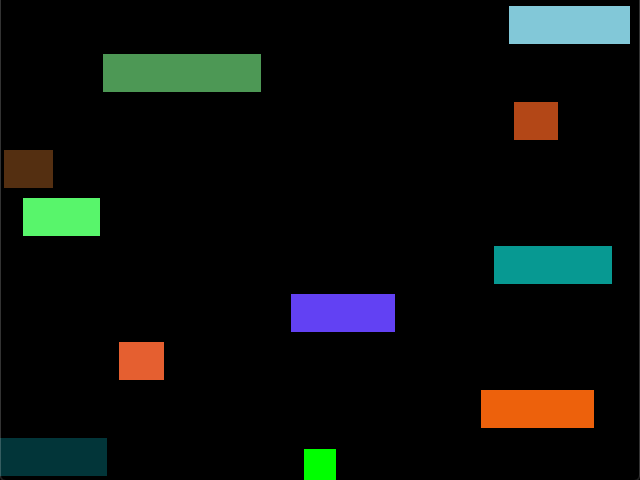
\includegraphics[width=.6 \textwidth]{conteudo/imgs/frogg_ini_state.png}
  \caption[Jogo \textit{Frogger}]{Exemplo do jogo \textit{Frogger} utilizado. O jogador controla o quadrado verde no centro inferior da tela, enquanto os outros retângulos coloridos são os obstáculos}
  \label{fig:frogg}
\end{figure} 

 As condições de parada, ou seja, os estados que constituem os estados finais do jogo são:

 \begin{itemize}
   \item Estados onde ocorra uma colisão do agente com o ambiente;
   \item Estado onde o agente atravessou o topo da tela (uma posição acima da última linha observável do jogo).
 \end{itemize}

 Por fim, as recompensas para ações durante o jogo foram definidas inicialmente da seguinte forma:

 \begin{itemize}
 	\item $r=-0.05$ caso o agente realize uma ação que o mantenha na mesma linha que se encontrava previamente. Essa recompensa negativa foi estipulada com o objetivo a desmotivar o agente a permanecer longos períodos de tempo sem progredir;
 	\item $r=1$ caso o agente realize uma ação que o aproxime verticalmente de seu objetivo;
  \item $r=-1$ caso o agente realize uma ação que o distancie verticalmente de seu objetivo;
 	\item $r=-1$ caso o agente realize uma ação que o leve a colidir com algum obstáculo (independente da direção que se movimentou);
 	\item $r=10$ caso o agente alcance seu objetivo.
 \end{itemize}

 % subsection o_jogo (end)
 
 \subsection{\textit{Allegro Learning Enviroment}} % (fold)
\label{sub:allegro_learning_enviroment}

Conforme descrito no \textbf{Capítulo \ref{chap:abordagem}}, será utilizada um \textit{Allegro Learning Enviroment} (ALE) que funcionará como intermédio entre o jogo e a IA. O ALE terá as seguintes funções principais:

\begin{itemize}
  \item Fornecer os valores de $\mathcal{A} = \{1,\cdots ,K\}$, que representa o conjunto de ações possíveis para o agente; 
  \item Determinar a posição da tela do jogo e realizar a captura das imagens que servirão como observações de estado para o agente;
  \item Executar um novo jogo para cada episódio de treinamento;
  \item Executar as ações estabelecidas pelo agente;
  \item Processar os dados do jogo incluindo: observação de cada instante de tempo, calcular a recompensa do atual estado do jogo, informação sobre quando um episódio é finalizado.
\end{itemize}

% subsection allegro_learning_enviroment (end)

% section reinforcement_learning (end)

\section{Modelagem Matemática} % (fold)
\label{sec:modelagem_matematica}

% \subsection{Aprendizagem por Reforço}

Conforme elaborado no \textbf{Capítulo \ref{chap:abordagem}}, no aprendizado por reforço, é desenvolvido um agente  um agente interage com um ambiente $\varepsilon$, nesse caso o jogo em \textit{Allegro}, como uma sequência de ações, observações e recompensas.
Em cada etapa de tempo, o agente seleciona uma ação em do conjunto de ações legais do jogo, $\mathcal{A} = \{1,\cdots ,K\}$. A ação é executada, modificando o estado do ambiente e pontuação do jogo.
%Em geral, $\varepsilon$ pde ser estocástico.
O estado interno do jogo não é observado pelo agente, este observa apenas uma imagem $x_t \in \mathbb{R}^d$, que é um vetor de valores de pixel brutos que representam a tela do estado atual do jogo. Além disso, o agente recebe uma recompensa $r$ que representa a alteração na pontuação do jogo.  

Em outras palavras, um agente explora um jogo, e é treinado tentando maximizar as recompensas nesse jogo. Este ciclo é ilustrado na \textbf{Figura \ref{rl-diagram-2}}.

\begin{figure}[h]
  \centering
  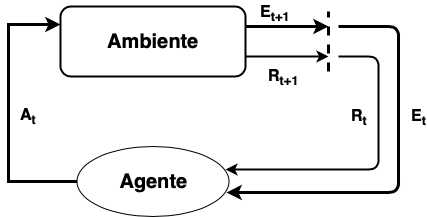
\includegraphics[width=.6 \textwidth]{conteudo/imgs/rl-diagram.png}
  \caption[Diagrama de aprendizagem por reforço]{Diagrama de aprendizagem por reforço elaborada melhor no \textbf{Capítulo \ref{chap:abordagem}}
  }
  \label{rl-diagram-2}
\end{figure}

% Em resumo, no \textit{loop} de \textit{feedback} mostrado na \textbf{Figura \ref{rl-diagram-2}}, os subscritos indicam as etapas de tempo $t$ e $t + 1$, cada uma das quais se refere a estados diferentes: o estado no momento $t$ e o estado no momento $t + 1$. 
% A ação $A_t$ de um agente é determinada por sua \textbf{política} $\pi$, que por sua vez é uma função que depende do estado atual do sistema $E_t$. A política de um agente tem como objetivo maximizar a \textbf{função de valor} $Q(s,a)$ que é calculada utilizando o \textbf{sinal de recompensa} $R_t$. O ambiente se comporta como um sistema caixa preta que transforma uma ação executada no estado atual $A_t$, no próximo estado $E_{t+1}$ e uma recompensa $R_{t+1}$

% \subsection{Processos de Decisão de Markov e a Equação de Bellman} % (fold)
% \label{sub:processos_de_decisão_de_markov}
% % subsection processo_de_decisão_de_markov (end)


É importante ressaltar que a pontuação do jogo pode depender de toda a sequência anterior de ações e observações. O feedback sobre uma ação só pode ser recebido depois de decorridos múltiplos de intervalos de tempo. Uma vez que o agente apenas observa as imagens da tela atual, a análise do atual estado do jogo pode ser mal-representada, ou seja, é difícil para o agente compreender totalmente a situação atual apenas da tela atual $x_t$. 
Para solucionar esse problema, considera-se como um estado $s_t$ do jogo, uma sequência de ações e observações $s_t = (x_{t-n},a_{t-n},\cdots,a_{t-1},x_t)$, as quais serão utilizadas para treinar o agente, fornecendo-o um melhor contexto do estado em que se encontra. Esse formalismo dá origem a um processo de decisão de Markov (MDP), no qual cada sequência é um estado distinto. Como resultado, podemos aplicar métodos de aprendizado por reforço padrão para MDPs, simplesmente usando a sequência completa $s_t$ como a representação do estado no tempo $t$.

Conforme descrito em \cite{play-atari-drl-deepmind}, o objetivo do agente é interagir com o jogo, selecionando ações de uma forma que maximize recompensas futuras. É feita a suposição padrão de que as recompensas futuras são descontadas por um fator de $\gamma$ por intervalo de tempo, e que o retorno descontado futuro é definido por: 
\begin{eqnarray}
	R_t=\sum_{t^{\prime}=t}^T \gamma^{t^{\prime}-t}\cdot r_{t^{\prime}}
\end{eqnarray}
onde T é o intervalo de tempo em que o jogo termina. 

A função de valor de ação ótima $Q^{*}(s, a)$ pode ser definida como o máximo retorno esperado alcançável de uma estratégia, depois de ver a sequência $s$ e se tomar alguma ação $a$:
\begin{eqnarray}
	Q^{*}(s, a)=max_\pi(\mathbb{E}[R_t | s_t=s,a_t=a,\pi])
\end{eqnarray}
onde $\pi$ é uma política que mapeia sequências para ações e $\mathbb{E}$ é a função de retorno esperado para um estado $s$ dado uma ação $a$.

A função de valor de ação ótima obedece a identidade da equação de Bellman. Essa se baseia na seguinte intuição: se o valor ótimo $Q^{*}(s_{t+1}, a_{t+1})$ da sequência $s_{t+1}$ na próxima etapa de tempo for conhecido para todas as ações possíveis ações $a_{t+1}$, então a estratégia ótima para o estado $s_t$ consiste em selecionar a ação $a_{t}$ que maximize o valor esperado futuro:

\begin{eqnarray}
	Q^{*}(s_t, a_t)= r + \gamma \cdot max(Q^{*}(s_{t+1},a_{t+1})|\forall a_{t+1})
\end{eqnarray}

A ideia básica por trás de muitos algoritmos de aprendizagem por reforço é estimar a função de valor de ação, usando a equação de Bellman como uma atualização iterativa. Assim, dado um fator de aprendizagem $\alpha$, o valor de $Q(s,a)$, é atualizado durante o treinamento da seguinte forma:

\begin{eqnarray}
  Q_{i+1}(s_t,a_t) = Q(s_t,a_t) + \alpha[r + \gamma\cdot max_{a_{t+1}}Q(s_{t+1},a_{t+1}) - Q(s_t,a_t)]
  \label{eq:qlearning}
\end{eqnarray}

sendo que a subtração de $\gamma\cdot max_{a_{t+1}}Q(s_{t+1},a_{t+1})$ por $Q(s_t,a_t)$ é realizada para normalizar a atualização. 

Essa atualização dos valores da função de valor $Q$, permite que o algoritmo convirja para a função de ação ótima $Q_i \rightarrow Q^*$, com $i\rightarrow\infty$ \cite{sutton-barto-rl-intro}. Na prática, essa abordagem é totalmente impraticável, pois a função valoração é estimada separadamente para cada sequência, sem nenhuma generalização. Em vez disso, é comum usar um aproximador de função para estimar a função de valor de ação, $Q(s,a;\theta_t) \approx Q^*(s,a)$. Este aproximador toma a forma de uma rede neural, conhecida como uma \textit{Q-network}, onde $\theta_t$ refere-se aos parâmetros da rede neural (ou seja, os pesos e bias da rede). Assim, se os pesos são atualizados após cada passo de tempo, então chegamos ao conhecido algoritmo de \textit{Q-learning} \cite{Watkins-Dayan-Qlearning}. O valor de $\theta_t$ por sua vex pode ser atualizado conforme a \textbf{Equação \ref{eq:theta}}:
\begin{eqnarray}
  \theta_t = \theta_t + \alpha(r + \gamma\cdot max_{a_{t+1}}Q(s_{t+1},a_{t+1}) - Q(s_t,a_t))\nabla_\theta Q(s_t,a_t)
  \label{eq:theta}
\end{eqnarray}

Por fim, considerando a iteração de treinamento do agente usando \textit{Q-learning}, a política de seleção de ação é baseada apenas no valor máximo de $Q$ em qualquer estado dado. É concebível que, dada a natureza aleatória do ambiente, o agente inicialmente tome decisões “ruins”. No entanto, como o agente nunca explorou ações melhores, ele pode interpretar que as decisões ruins tomadas inicialmente são boas e, daquele momento em diante, tomar somente aquelas decisões. Da mesma forma, mesmo que o agente tome ações iniciais ``boas'' ele pode acabar desenvolvendo uma política que prenda o agente em ótimos locais, ou seja, a ação determinada pela política é boa a curto prazo, mas a longo prazo ela é inferior ou até ruim. Esta política de seleção de ação é chamada de política gulosa.

Para evitar esses problemas, o agente deve explorar o maior número possível de estados e ações. Infelizmente, para problemas com um número muito grande de estados, explorar todos os estados e ações possíveis se torna impraticável. A política \textit{epsilon-greedy} na aprendizagem por reforço é basicamente a mesma que a política gulosa, exceto que há um valor épsilon que define uma probabilidade $1-\epsilon$ de uma ação ser escolhida aleatoriamente ao invés de definida pelo atual modelo. Dessa forma, o algoritmo força o agente a explorar diversos estados e ações, mesmo que estes não sejam a princípio recomendados pela função de valor $Q$. Dado um número suficientemente grande de ações, o agente terá explorado uma quantidade de estados suficiente para determinar uma política satisfatória. Essa abordagem permite também que o valor de $\epsilon$ seja atualizado e reduzido com o tempo de forma a permitir que o algoritmo se concentre mais em explorar as melhores soluções que encontrou. 

% section modelagem_matemática (end)

\section{Implementação} % (fold)
\label{sec:implementacao}

% \begin{algorithm}[H]
% \SetAlgoLined
% \Inicio{
%   Inicializa memória de experiência $\mathcal{D}$ com capacidade $N$\\
%   Inicializa função de valor de ação $Q$ com pesos aleatórios
%   \\
%   \For{episodio=1:MAX\_NUM\_EPISODIOS}{
%     Inicializa o estado $s_1 = \{x_1\}$ \\
%     Inicializa a função $\phi_1=\phi(s_1)$\\
%     $t=1$
%     \While{episodio não chegou ao fim}{
%       Com uma probabilidade de $\epsilon$ selecione uma ação aleatória $a_t$, caso contrário selecione $a_t=max_aQ^*(\phi(s_t),a;\theta)$\\

%       Execute a ação $a_t$ e receba a recompensa $r_t$ e a imagem $x_{t+1}$

%       Defina o próximo estado $s_{t+1}=s_t,a,x_{t+1}$\\
%       Defina $\phi_{t+1}=\phi(s_{t+1})$

%       $t++$;
%     }
%   }
% }
%  \caption{\textit{Deep Q-learning}}
% \end{algorithm}

A modelagem descrita na \textbf{Seção \ref{sec:modelagem_matematica}}, fornece uma modelagem da rede neural proposta. No entanto, um simples algoritmo usando o método \textit{Q-learning} descrito não converge para uma solução satisfatória. Nessa seção serão vistas algumas modificações para o algoritmo que o fará obter melhores resultados.


Foi aplicada a técnica conhecida como \textit{Experience Replay} \cite{Lin1992ReinforcementLF},
 % onde as experiências do agente em cada passo de tempo, $e_t = (s_t, rt, st + 1)$ são armazenadas em um conjunto de dados D = e1, ... , eN, agrupados ao longo de muitos episódios em uma memória de repetição. Durante o loop interno do algoritmo, aplicamos atualizações de Q-learning, ou atualizações de minibatch, a amostras de experiência, e ∼ D, retiradas aleatoriamente do pool de amostras armazenadas. Após realizar a repetição da experiência, o agente seleciona e executa uma ação de acordo com uma política ε-greedy. Visto que usar histórias de comprimento arbitrário como entradas para uma rede neural pode ser difícil, nossa função Q em vez disso trabalha na representação de comprimento fixo de histórias produzidas por uma função φ.


\subsection{Pré-processamento de Dados} % (fold)
\label{sub:preprocessamento}

% subsection préprocessamento (end)


\subsection{Limitações} % (fold)
\label{sub:limitacoes}

A implementação do sistema apresentado enfrentou uma série de limitações que fogem do alcance do desenvolvedor. Os desafios encontrados durante a implementação, assim como as soluções para circunver estes problemas, quando possível, são descritas abaixo.

\subsubsection{Tempo de Treinamento e Limitações de Hardware} % (fold)
\label{subsub:tempo_de_treinamento_e_limitações_de_hardware}

O principal obstáculo enfrentado foi o tempo de treinamento do sistema. Devido a complexidade e número de entradas do problema, o modelo pode levar dias ou semanas para alcançar uma política ótima. Como mencionado anteriormente, cada estado é formado por quatro imagens constituindo os quatro últimos instante do jogo. Mesmo após a conversão para cinza e compressão das imagens de $640\times480$ para $84\times84$ pixels, isso ainda deixa cada estado com um vetor de entrada de tamanho $84\times84\times4=28224$. Tudo isso considerando um tamanho de tela bem modesto e um jogo sem informações muito complexas (quando comparado com um jogo 3D por exemplo).

Esses problemas são agravados ainda mais devido às limitações do hardware onde o sistema foi implementado. A máquina utilizada possui as seguintes especificações:

\begin{itemize}
  \item MacBook Air 2015;
  \item Processador: 1.6 GHz Dual-Core Intel Core i5;
  \item Memória: 4 GB 1600 MHz DDR3;
  \item Sistema Operacional: macOS Catalina.
\end{itemize}

Como pode ser observado, trata-se de uma máquina com poder computacional limitado, com relativamente pouca memória, um processador bastante simples e sem uma placa de vídeo dedicada. Todas essas limitações acabam levando à um tempo de treinamento ainda maior.

% subsection tempo_de_treinamento_e_limitações_de_hardware (end)

\subsubsection{Integração do Sistema com o Jogo em \textit{Allegro}} % (fold)
\label{subsub:integração_do_sistema_com_o_jogo}

Como mencionado no \textbf{Capítulo \ref{chap:abordagem}} e em \ref{sub:allegro_learning_enviroment}, a comunicação entre a IA, implementada em \textit{Python}, e o jogo, implementado em C, é realizada através de um \textit{Allegro Learning Enviroment} (ALE). No entanto, como o ALE também é implementado em \textit{Python}, a integração dos dois sistemas sofre algumas limitações.

Primeiramente, o cálculo da recompensa seria, idealmente, calculado pelo programa do jogo e passado para o ALE. No entanto, qualquer saída do programa em C só é recebida pelo ALE uma vez que o programa é finalizado ao fim de um episódio. Isso inviabiliza o calculo em tempo real de qualquer estado que não sejam os estados iniciais ou finais. Por esse motivo o calculo das recompensas de cada estado deve ser feito pela ALE, o qual é realizado através um simples registro da posição do agente no jogo.

Outro problema que surge da integração da ALE com o o jogo é o processamento das imagens e que, por sua vez, acaba exacerbando ainda mais o problema de tempo de treinamento descrito em \ref{subsub:tempo_de_treinamento_e_limitações_de_hardware}. Ao iniciar um novo episódio, o programa em C leva alguns instantes para ser lançado e ter seu estado inicial renderizado. Portanto, para garantir que a observação do estado inicial do jogo seja realizada propriamente, a ALE aguarda $0.1s$ para garantir que o programa foi inicializado propriamente. Esse tempo torna-se considerável a medida que o número de episódios de treinamento aumentam. Um trinamento com dez mil episódios, por exemplo, recebem um aumento de tempo maior do que $16min$. 

Além disso, diferente de jogos em Atari 2600 que possuem um emulador em \textit{Python} que é capaz de gerar um vetor de observação que contém os dados de cada instante do jogo sem a necessidade de renderizar as imagens do mesmo \cite{brockman2016openai}, os jogos em \textit{Allegro} devem ter seus dados processados manualmente. Isso inclui executar o programa em C, renderizar cada estado do jogo e realizar a captura de tela dos mesmos, e realizar o processamento dessas imagens antes desses dados serem passados para a IA. A \textbf{Figura \ref{fig:process_img}} mostra um diagrama que indica todos os passos do processamento de dados necessários para gerar as informações de cada estado do jogo.

\begin{figure}[h]
  \centering
  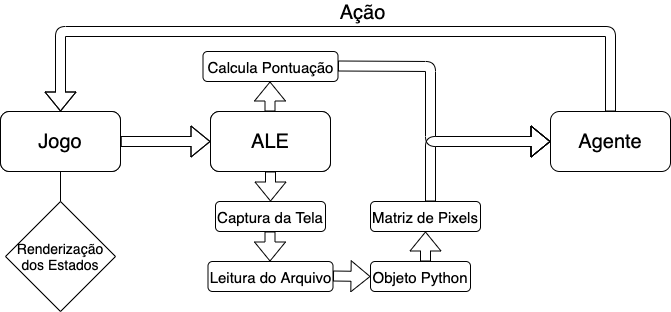
\includegraphics[width=.8 \textwidth]{conteudo/imgs/processamento_imgs.png}
  \caption[Diagrama de processamento de imagens]{Diagrama mostrando como as informações de cada estado são processadas antes de serem passadas para a IA. Isso inclui executar o programa em C, transmitir os comandos de ação do agente para o jogo, renderizar as imagens em cada instante do jogo, realizar a captura de tela, acessar os arquivos onde essas imagens foram salvas, transformar os dados desse arquivo para um objeto em \textit{Python}, transformar o objeto em uma matriz com os dados da imagem para somente então os mesmos serem passados para o modelo a ser treinado}
  \label{fig:process_img}
\end{figure} 

Lembrando que todo o processo indicado na \textbf{Figura \ref{fig:process_img}} deve ser realizado para cada instante que deseja-se observar e calcular uma ação. Para evitar que o alto tempo de processamento dos dados leve a alguma perda de informações que prejudique o treinamento (como o agente permanecer inativo por um longo período de tempo enquanto calcula o próximo movimento), o jogo foi alterado de forma que cada quadro (\textit{frame}) do jogo seja atualizado somente quando o agente realizar uma ação. Esse formato de implementação acaba constituindo um \textit{trade-off}: a perda de informações do agente é minimizada, mas o tempo de execução de cada episódio aumenta.

% subsection integração_do_sistema_com_o_jogo_em_tex (end)

% subsection limitações (end)
% section implementação (end)
